\chapter[Comparison of Methods for Estimating Groundwater Budgets in an Agriculturally-Intensive Alluvial Aquifer System]{Comparison of Methodologies for Estimating Groundwater Budgets in an Agriculturally-Intensive Alluvial Aquifer System.\footnote[1]{Portions of this chapter have been submitted to \textit{Journal of Environmental Management}: Escriva-Bou, A; Hui, R.; Maples S.R.; Medellín-Azuara, J.; Harter, T; Lund, J.R. ``Planning for Groundwater Sustainability Accounting for Uncertainty and Costs: an Application to California's Central Valley''.  (Submitted Aug. 2019)}}

\section{Abstract}

\noindent Data availability for groundwater pumping and storage is poor in many semi-arid, agriculturally-dominated groundwater systems, which presents challenges for estimating groundwater budgets and ensuring groundwater sustainability. This is especially true in California's Central Valley, which comprises a vast interconnected aquifer system with complex surface water routing networks and poor historical measurements of groundwater pumping and heads. To estimate groundwater budgets in these systems, most approaches rely on agricultural (i.e., landscape) water balance methods of varying complexity that require data on surface water deliveries, crops, weather, and climate to estimate crop water demand and calculate demand for agricultural groundwater pumping, which is fundamentally estimated as the residual of combined surface water and precipitation deliveries minus crop water demand and irrigation efficiency. Iteratively-coupled models, including the Integrated Water Flow Model (IWFM) and MODFLOW Farm Process (MF-FMP2) are commonly used to link a groundwater model with an agricultural water balance model. Coupling agricultural and groundwater components can, in theory, more accurately simulate feedbacks between climate, agricultural, vadose-zone, and groundwater processes and simulate phenomena on crops such as soil-moisture-deficit impacts and direct groundwater uptake, but there is uncertainty regarding the degree of complexity necessary to conceptualize and parameterize these processes. Here, we compare results from IWFM and MF-FMP2 water budget estimates at the supra-regional, regional, and subregional scale in the Central Valley during a concurrent 42-year period. Results show varied agreement for water budget components between models, with generally better agreement at larger spatial scales and for aggregated water budget components. Model agreement generally decreases for smaller spatial scales, especially in the Northern Central Valley, and for more granular, individual water budget components. Systematic biases reflecting the partitioning of outflows from the landscape systems were observed between models and appear to be related to differences in model’s physical conceptualization of processes other than the goundwater flow equation that control the boundary conditions for the latter. Some differences were also observed for input data that ostensibly are derived from similar or identical sources and likely contribute to differences in simulated output discrepancies.

\section{Introduction}

The Central Valley’s vast interconnected aquifer system and complicated network of land use and surface water routing creates challenges for estimating water budgets \citep{hanak_managing_2011}. System complexity is compounded by a lack of historical groundwater level measurements and groundwater pumping data \citep{harter2008legal}. Where comprehensive monitoring is lacking, accurate estimation of the groundwater budget remains challenging, and information gaps limit effective groundwater-resource management by policy makers \citep{hanak_managing_2011}. Overdraft estimates for the Central Valley are inherently uncertain given hydrological variability and uncertinaty in estimating aquifer characteristics, groundwater inflows, recharge, pumping, stream depletion, and connections with nearby aquifers. Reported estimates of overdraft rates in the Central Valley range from 1.3--9.0 million acre-ft yr$^{-1}$ for different periods and assessment methods \citep{brush2013development,hanak2018replenishing,famiglietti2011satellites,faunt2009groundwater,xiao2017much}.

Methods for simulating water budgets in agriculturally-dominated groundwater systems typically rely on crop-irrigation accounting methods of varying complexity usually involving an uncoupled or iteratively coupled groundwater model. Uncoupled agricultural water balance models are used extensively in semi-arid agricultural basins, with unquantified groundwater pumping and recharge treated as closure terms for the land-surface water budget \citep{belitz1993numerical,ruud2004estimation}. Coupled models, such as the Integrated Water Flow Model (IWFM) \citep{dogrul2012integrated} and MODFLOW Farm Process (MF-FMP2) \citep{schmid2006user} are common, with iteratively-coupled codes linking a groundwater model with an agricultural water balance model. Coupling agricultural and groundwater components can, in theory, more accurately simulate feedbacks between agricultural, vadose, and groundwater processes and simulate crop processes such as soil-moisture-deficit and direct groundwater uptake. Both uncoupled and coupled approaches require data on crops, weather, and climate to estimate crop water demand, and they require surface water delivery estimates to calculate demand for groundwater pumping. When measured or reported pumping data is absent, agricultural groundwater pumping is fundamentally estimated as the residual of combined surface water and precipitation deliveries minus crop water demand and irrigation efficiency. The main input data for the agricultural water components of each model are generally the same: crop information, weather and climate data, and surface water deliveries. 

In the past, the choice of numerical groundwater modeling code to simulate a groundwater flow problem was largely inconsequential, in that resulting computed hydraulic heads and water budgets were not very dependent on the choice of the code, as long as the data inputs (i.e., aquifer properties, initial and boundary conditions) were similar. For well known initial and boundary conditions, all solve the governing groundwater flow equation, and yield comparable results when discretized and parameterized similarly \citep{wang1977finite,anderson2015applied}, regardless of whether they are formulated as finite difference or finite element. However, coupled agricultural groundwater models like IWFM and MF-FMP that are used to simulate agricultural water demand not only solve the groundwater flow equation, but also employ varied conceptual and mathematical representations of land-surface and soil zone processes, most notably in the methods for estimating water supplied to and consumed by agricultural and natural plants. These, in turn control the boundary conditions for the groundwater flow problem. Consequently, large uncertainty appears to be related directly to the choice of code. These differences obfuscate the scientific value of these models. At best, model discrepancies reflect, and may help bracket, the true uncertainty of Central Valley water budgets; at worst, the differences reflect model bias stemming from poor understanding and/or representation of the fundamental physical processes. This is a research problem that demands further scientific scrutiny.

Several studies have highlighted the methodological differences between IWFM and MF-FMP2 in hypothetical settings \citep{harter2013peer,dogrul2011integrated,schmid2011comparison}, but none are diagnostic of how model differences affect the assessment of future conditions in applied settings. These studies show that conceptual differences between these codes primarily relate to the partitioning of ET requirements, representation of soil-moisture conditions, and prioritization of water allocation. For instance, MF-FMP2 assumes steady-state soil-moisture conditions, while IWFM simulates transient soil-moisture storage conditions. The MF-FMP2 and IWFM methodologies have each been separately applied for the Central Valley to estimate historical groundwater budgets \citep{brush2013development,faunt2009groundwater}. These models, named CVHM and C2VSim, were developed by the U.S. Geological Survey (USGS) and California Department of Water Resources (DWR), respectively \citep{faunt2009groundwater,brush2013development}. Preliminary investigations have shown that water budgets and storage estimates are significantly different for each model, especially at the sub-regional scale that is important for water management \citep{chou2012groundwater, maples2015estimation}. 

Broadly, this research aims to fill scientific knowledge gaps related to estimating groundwater pumpage and recharge processes in agriculturally-dominated groundwater basins. Specifically, this work reviews estimates of landscape and groundwater budgets for two regional-scale groundwater models of California's Central Valley, CVHM and C2VSim. This work examines two related, fundamental scientific questions: (1) To what extent can unmeasured water budget components (i.e., agricultural groundwater pumping) in agriculturally-dominated groundwater systems be constrained with a combination of agricultural irrigation accounting methods and groundwater models? (2) Do methodological or conceptual differences contribute to differences in water budget estimates in CVHM and C2VSim? That is to say, to what degree do the differences in water budget estimates reflect propagation of the inherent parametric uncertainty of input data (i.e., data on crops, weather and climate, and surface water deliveries) or structural uncertainty of the methods, which may oversimplify, omit, or misrepresent important physical processes? 

%%% MATERIALS & METHODS %%%
\section{Materials and Methods}
\subsection{Estimates of Groundwater Balance Components of California’s Central Valley}

The Central Valley aquifer system includes three interconnected regional aquifers (i.e., the Sacramento Valley, San Joaquin Valley, and Tulare Lake aquifers). The California Department of Water Resources (DWR) has additionally designated 21 aquifer sub-regions within this Central Valley aquifer system (Fig. \ref{fig:ch3_regions}). CVHM and C2VSim provide estimates of historical hydrologic budgets for each of these subregions during an overlapping, multi-decadal simulation period from 1962-2003. This spatial and temporal overlap aids in estimating the effects of methodological differences between models on the estimation of regional and sub-regional water budgets. The models use some similar data for precipitation, surface water inflows, and surface water diversion volumes \citep{dogrul2011integrated}, as well as identical estimates for urban groundwater pumping \citep{brush2013development, faunt2009groundwater}.

%% FIG Regions and subregion overview figure  
\begin{figure}[ht!]
\centerline{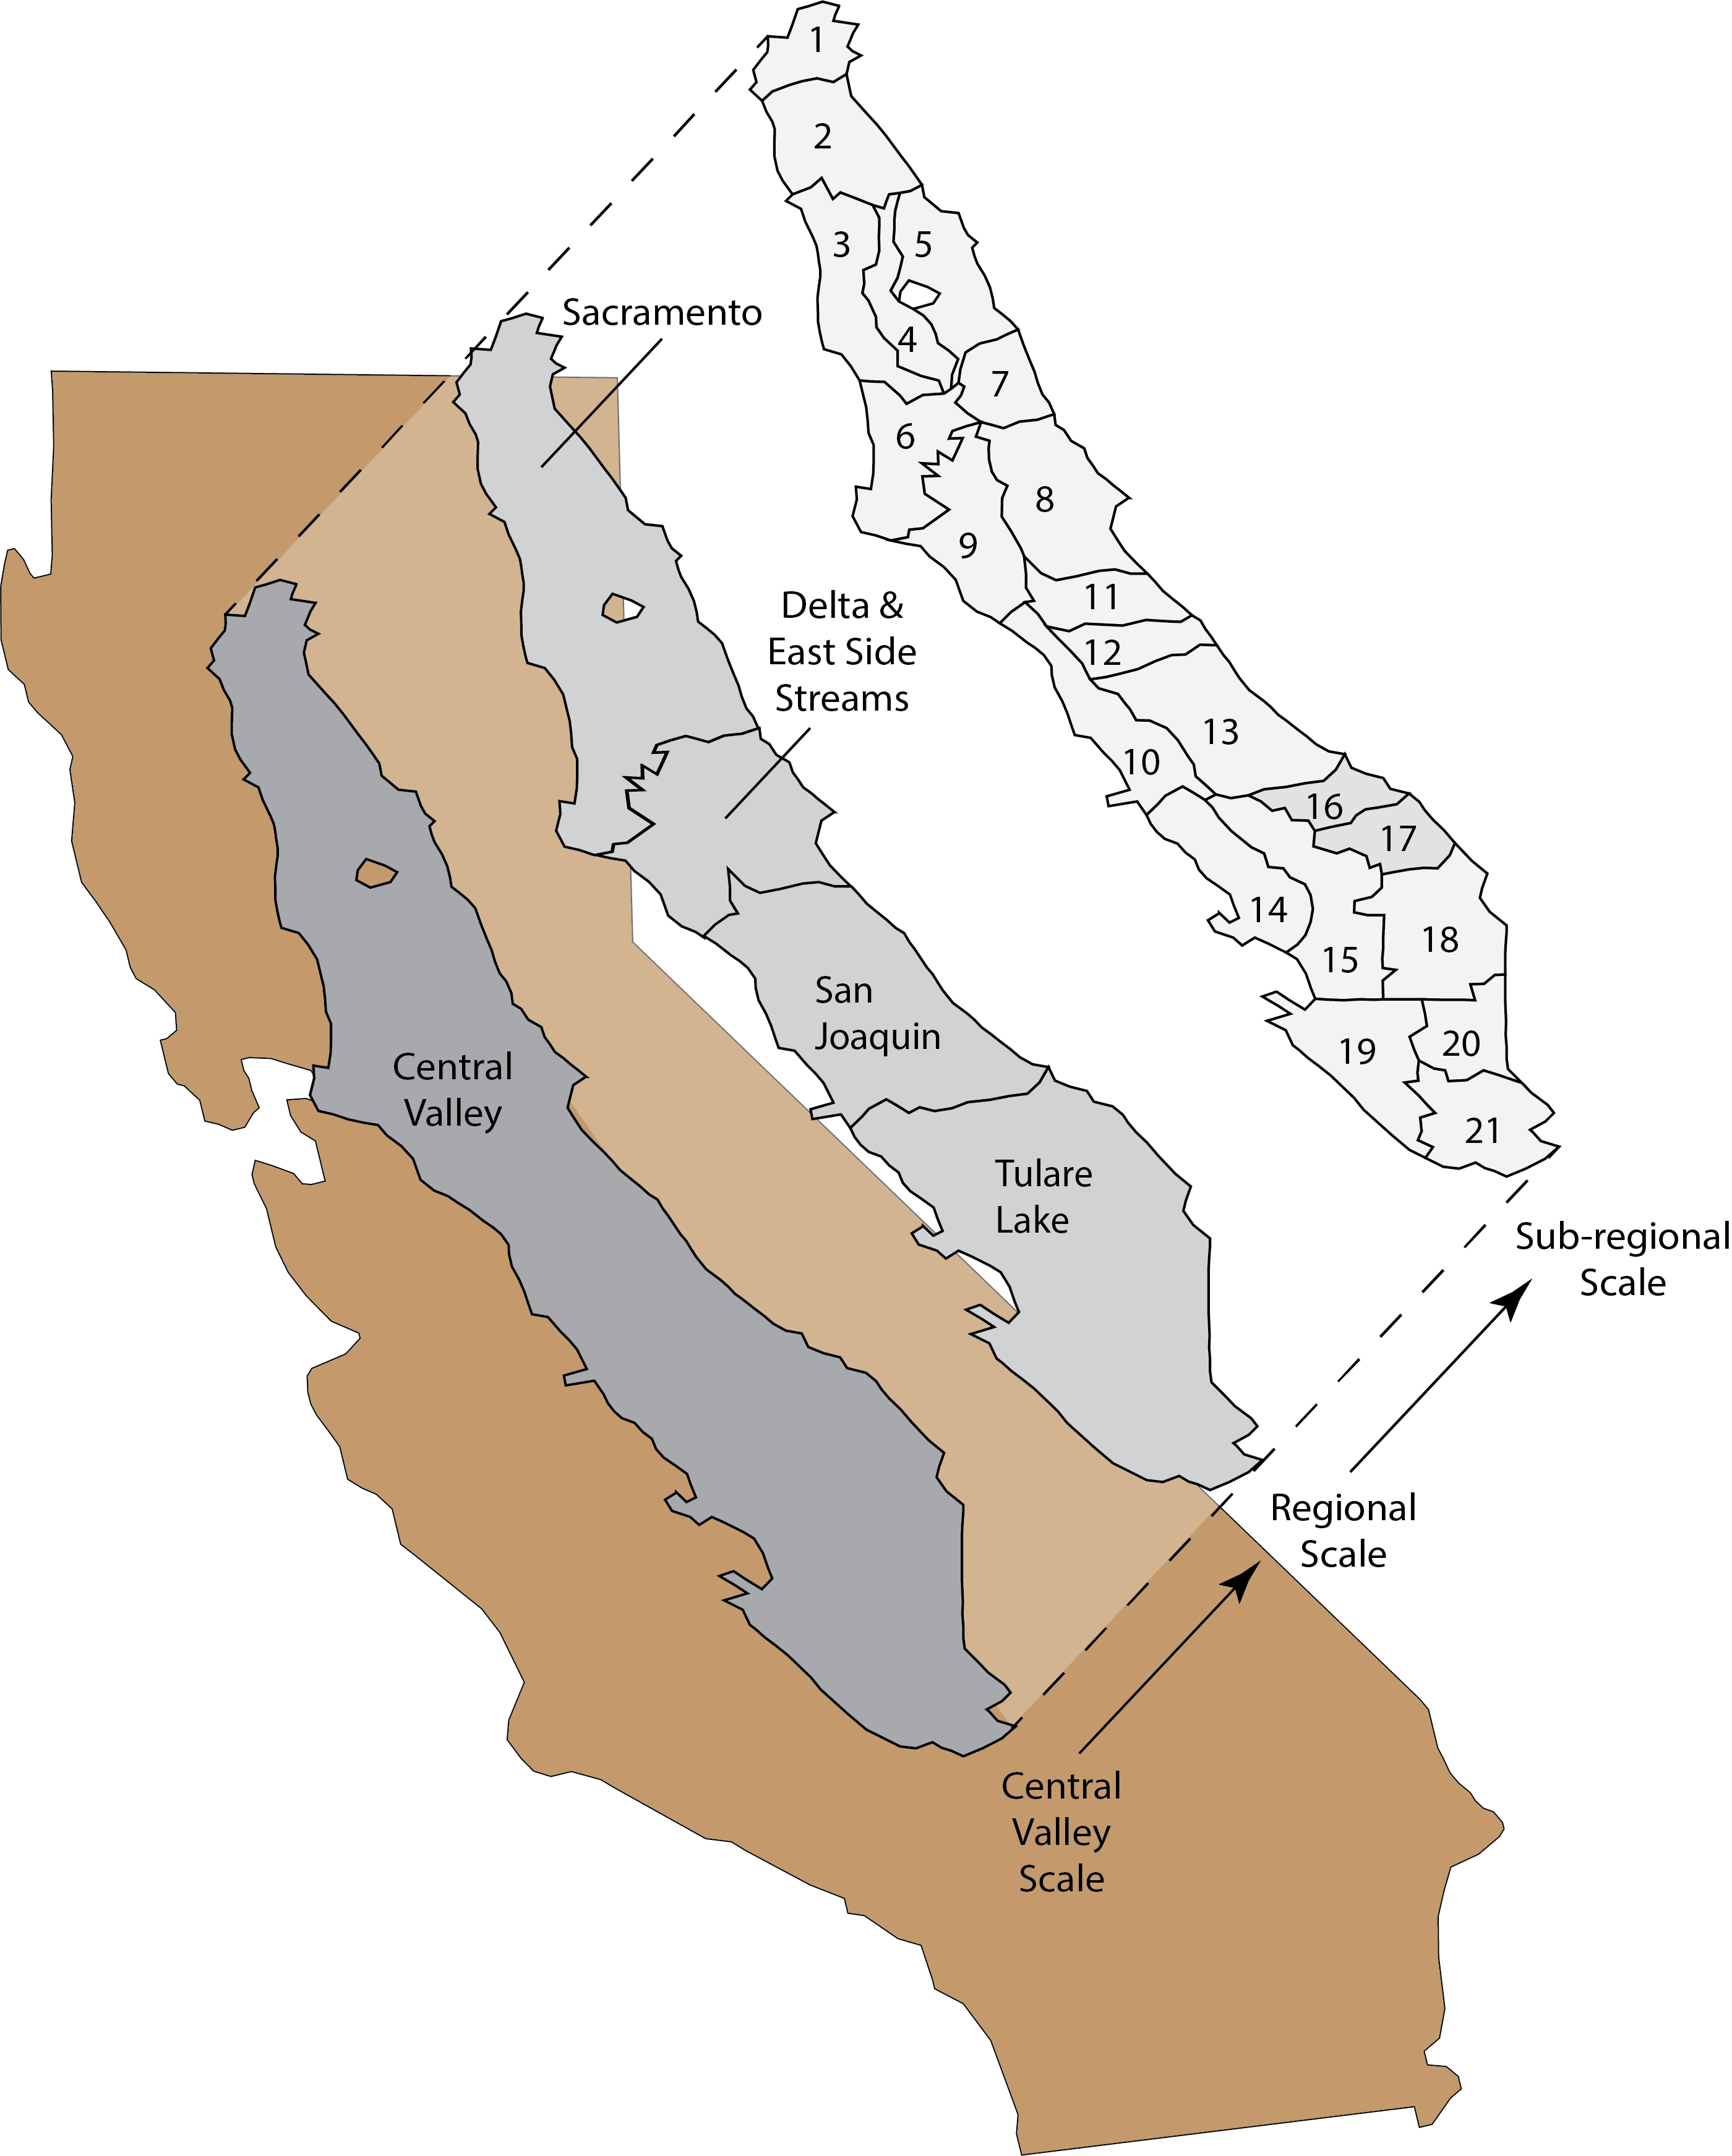
\includegraphics[width=100mm,keepaspectratio]{ch3_figs/CV_subregions_fig_Alvar_040819.png}}
\caption{Spatial extent of sub-regional, regional, and supra-regional areas used for model comparison.}
\label{fig:ch3_regions}
\end{figure}

\subsection{Major Water Balance Components}

Simulated model outputs from CVHM and C2VSim were aggregated to estimate the major flow components into and out of the landscape and groundwater systems in each model (Fig. \ref{fig:ch3_conceptual}a). Because IWFM and MF-FMP2 have some important conceptual differences, the major flow components are comprised of various individual water flow components that are output by each model (Fig. \ref{fig:ch3_conceptual}b-e; Tables \ref{table:ch3_LS_flow_components},\ref{table:ch3_GW_flow_components}) and are described in detail for CVHM in Tables \ref{table:ch3_CVHM_LS}, and \ref{table:ch3_CVHM_GW}, as well as for C2VSim in Tables \ref{table:ch3_C2VSim_LS}, and \ref{table:ch3_C2VSim_GW}. In general, IWFM partitions flow components according to land use in C2VSim for landscape water budgeting, whereas MF-FMP2 does not generally partition outputs according to land use, but instead partitions outputs according to physical processes. For example, MF-FMP2 partitions ET by process into individual evaporation and transpiration components for irrigation, precipitation, and groundwater in CVHM (Fig. \ref{fig:ch3_conceptual}b), whereas IWFM partitions ET by land-use designation (i.e., agricultural, urban, and native/riparian areas; Fig. \ref{fig:ch3_conceptual}c).

%% FIG Landscape and GW components conceptual model    
\begin{figure}[ht!]
\centerline{\includegraphics[width=150mm,keepaspectratio]{ch3_figs/Landscape_system_compare_ALLcompact_082919.pdf}}
\caption{Conceptual model showing (a) the major groundwater and landscape water budget components used for model comparison, as well as individual water budget variables for CVHM (b) and C2VSim (c) landscape systems and CVHM (d) and C2VSim (e) groundwater systems.}
\label{fig:ch3_conceptual}
\end{figure}

For the landscape system, fluxes into and out of any given landscape area can be generalized into major flow components that include precipitation, surface diversions, evapotranspiration (ET), runoff and return flows, and deep percolation. For the purposes of this study, the total flows into the landscape system are given as 

%landscape in
\begin{equation}
\begin{aligned}
Total \; Landscape \; (in) ={} & Precipitation \; (in) \\
& + Groundwater \; Pumping \; (in) \\
& + Surface \; Water \; Diversions \; (in)
\end{aligned}
\end{equation}

\noindent and the total flows out of the landscape system are given as

%landscape out
\begin{equation}
\begin{aligned}
Total \; Landscape \; (out) ={} & Evapotranspiration \; (out) \\
& + Runoff \; \& \; Return \; Flow \; (out) \\
& + Deep \; Percolation \; (out)
\end{aligned}
\end{equation}

\noindent where each flow component comprises CVHM and C2VSim variables described in Table \ref{table:ch3_LS_flow_components}.

%% TABLE of landscape variables
\input{ch3_tables/Landscape_Flow_components.tex}

For the groundwater system, fluxes into and out of any groundwater area can be generalized into flow components that include exchanges with surface water and the landscape, subsurface exchanges with adjacent groundwater areas, and groundwater pumping. For the purposes of this study, the total flows into the groundwater system are given as 

%groundwater in
\begin{equation}
\begin{aligned}
Total \; Groundwater \; (in) ={} & Surface \; Water \; Gains \; (in) \\
& + Landscape \; Recharge \; (in) \\
& + Net \; Boundary \; Inflows \; (in)
\end{aligned}
\end{equation}

\noindent and the total flows out of the landscape system are given as

%groundwater out
\begin{equation}
\begin{aligned}
Total \; Groundwater \; (out) ={} & Surface \; Water \; Losses \; (out) \\
& + Groundwater \; Pumping \; (out) \\
& + Net \; Boundary \; Outflows \; (out)
\end{aligned}
\end{equation}

\noindent where each flow component comprises CVHM and C2VSim variables described in Table \ref{table:ch3_GW_flow_components}.

%% Table of groundwater variables
\input{ch3_tables/GW_Flow_components.tex}

Annual water budget volumes were calculated for each major landscape and groundwater flow component at the supra-regional, regional, and subregional scales for each model during a concurrent simulation period from water years 1962--2003. Water budget values were gathered from model output files and were parsed at to the regional and subregional scales with the ZONEBUDGET and Z-Budget post-processing packages for MODFLOW and IWFM, respectively. In C2VSim, groundwater pumping outputs are partitioned by land use, so urban or agricultural groundwater pumping volumes were easily differentiated. In CVHM, however, model outputs are generally not partitioned by land use. Fortunately, urban pumping is specified in both models using identical values for each subregion \citep{brush2013development,faunt2009groundwater}, so any variation in estimated total pumping is due to differences in estimated agricultural groundwater pumping alone.

In addition to major landscape and groundwater flow components described above, total annual groundwater storage values were gathered for both models to compare groundwater storage trends. Average annual groundwater storage trends for each model during 1962--2003 were calculated using linear regression. Area-averaged groundwater change-in-storage trends were compared using the respective linear regression for each model.

\subsection{Water Budget Comparison Methods}

To evaluate differences in annual water budgets between CVHM and C2VSim, several statistical analyses were applied. Specifically, the root mean square error ($RMSE$), Pearsons $r$, and mean bias error ($MBE$) statistics were calculated on annual volumes of each generalized landscape and groundwater flow component for each model during water years 1962--2003. In order to compare these statistics for different flow components and across spatial scales, flow components for each model were normalized according to 

%normalization eqn
\begin{align}
X_{norm, i} = \frac{X_i}{X_{max}} && Y_{norm, i} = \frac{Y_i}{Y_{max}}
\end{align}

\noindent where $X_i$ and $Y_i$ are annual volumes of flow components from CVHM and C2VSim, respectively, and $X_{norm,i}$ and $Y_{norm,i}$ are the values normalized by the maximum values $X_{max}$ and $Y_{max}$. Flow components, $X_i$ and $Y_i$ are net values that are partitioned such that flows into and out of the landscape and groundwater systems are all represented as positive values. For example, if a surface water system has a net loss during one year, this is represented as a single positive inflow to the groundwater system, with no corresponding outflow from the groundwater system. Conversely, if the surface water system is gaining in another year, it is represented as a positive outflow from the groundwater system with no corresponding inflow.  Accordingly, normalized $RMSE$, normalized Pearsons $r$ , and normalized $MBE$ are each calculated as follows

%Normalized RMSE
\begin{equation}
RMSE = \sqrt{\frac{1}{n}\sum\limits_{i=1}^{n}{(X_{norm, i} -Y_{norm, i})^2}}
\end{equation}

%Pearsons r
\begin{equation}
r = \frac{\sum\limits_{i=1}^{n}{(X_{norm, i} -\bar{X}_{norm})}{(Y_{norm, i} -\bar{Y}_{norm})}}{\Bigg\{\sum\limits_{i=1}^{n}{(X_{norm, i} -\bar{X}_{norm})^2}\sum\limits_{i=1}^{n}{(Y_{norm, i} -\bar{Y}_{norm})^2}\Bigg\}^{1/2}}
\end{equation}

%Normalized mean bias
\begin{equation}
MBE = \frac{1}{n}\sum\limits_{i=1}^{n}{(X_{norm, i} -Y_{norm, i})}
\end{equation}

This combination of statistics provides various measures of agreement between each model. $RMSE$ describes the absolute agreement of values along the 1:1 line, ranging from 0 to 1 when calculated with normalized values $X_{norm,i}$ and $Y_{norm,i}$, where 0 indicates perfect agreement. Pearsons $r$ describes the linear correlation between the values, ranging from 0 to 1, where 1 indicates perfect correlation and 0 indicates no correlation. $MBE$ describes model bias, ranging from 0 to 1, where 0 indicates no model bias.

\subsection{Comparison of Model Hydraulic Properties}

Differences in the distribution vertical and horizontal hydraulic conductivity ($K$) were compared for coincident model layers in each model (Fig. \ref{fig:ch3_model_layers}) at the supra-regional, regional, and subregional scales. C2VSim represents the groundwater system with 4 model layers, while CVHM uses 10 model layers. The Corcoran clay, a laterally-continuous fine-texture confining layer that is present in the majority of the Tulare region and parts of the San Joaquin region, is represented in model layer 2 and layers 4--5 in C2VSim and CVHM, respectively, where it is present. Layer 1 and layers 1-3 represent the uppermost coincident model layers that overly the Corcoran clay (where present) in C2VSim and CVHM, respectively, while layers 3--4 and layers 6--10 represent sediments underlying the Corcoran clay (where present). For the purposes of this comparison, layer 3 and layers 6--7 as well as layer 4 and layers 8--10 were treated as coincident in C2VSim and CVHM, respectively. C2VSim does not simulate lateral groundwater flow through the Corcoran clay, so comparison of horizontal $K$ was not conducted for these layers.

%% FIG GW model layers
\begin{figure}[ht!]
\centerline{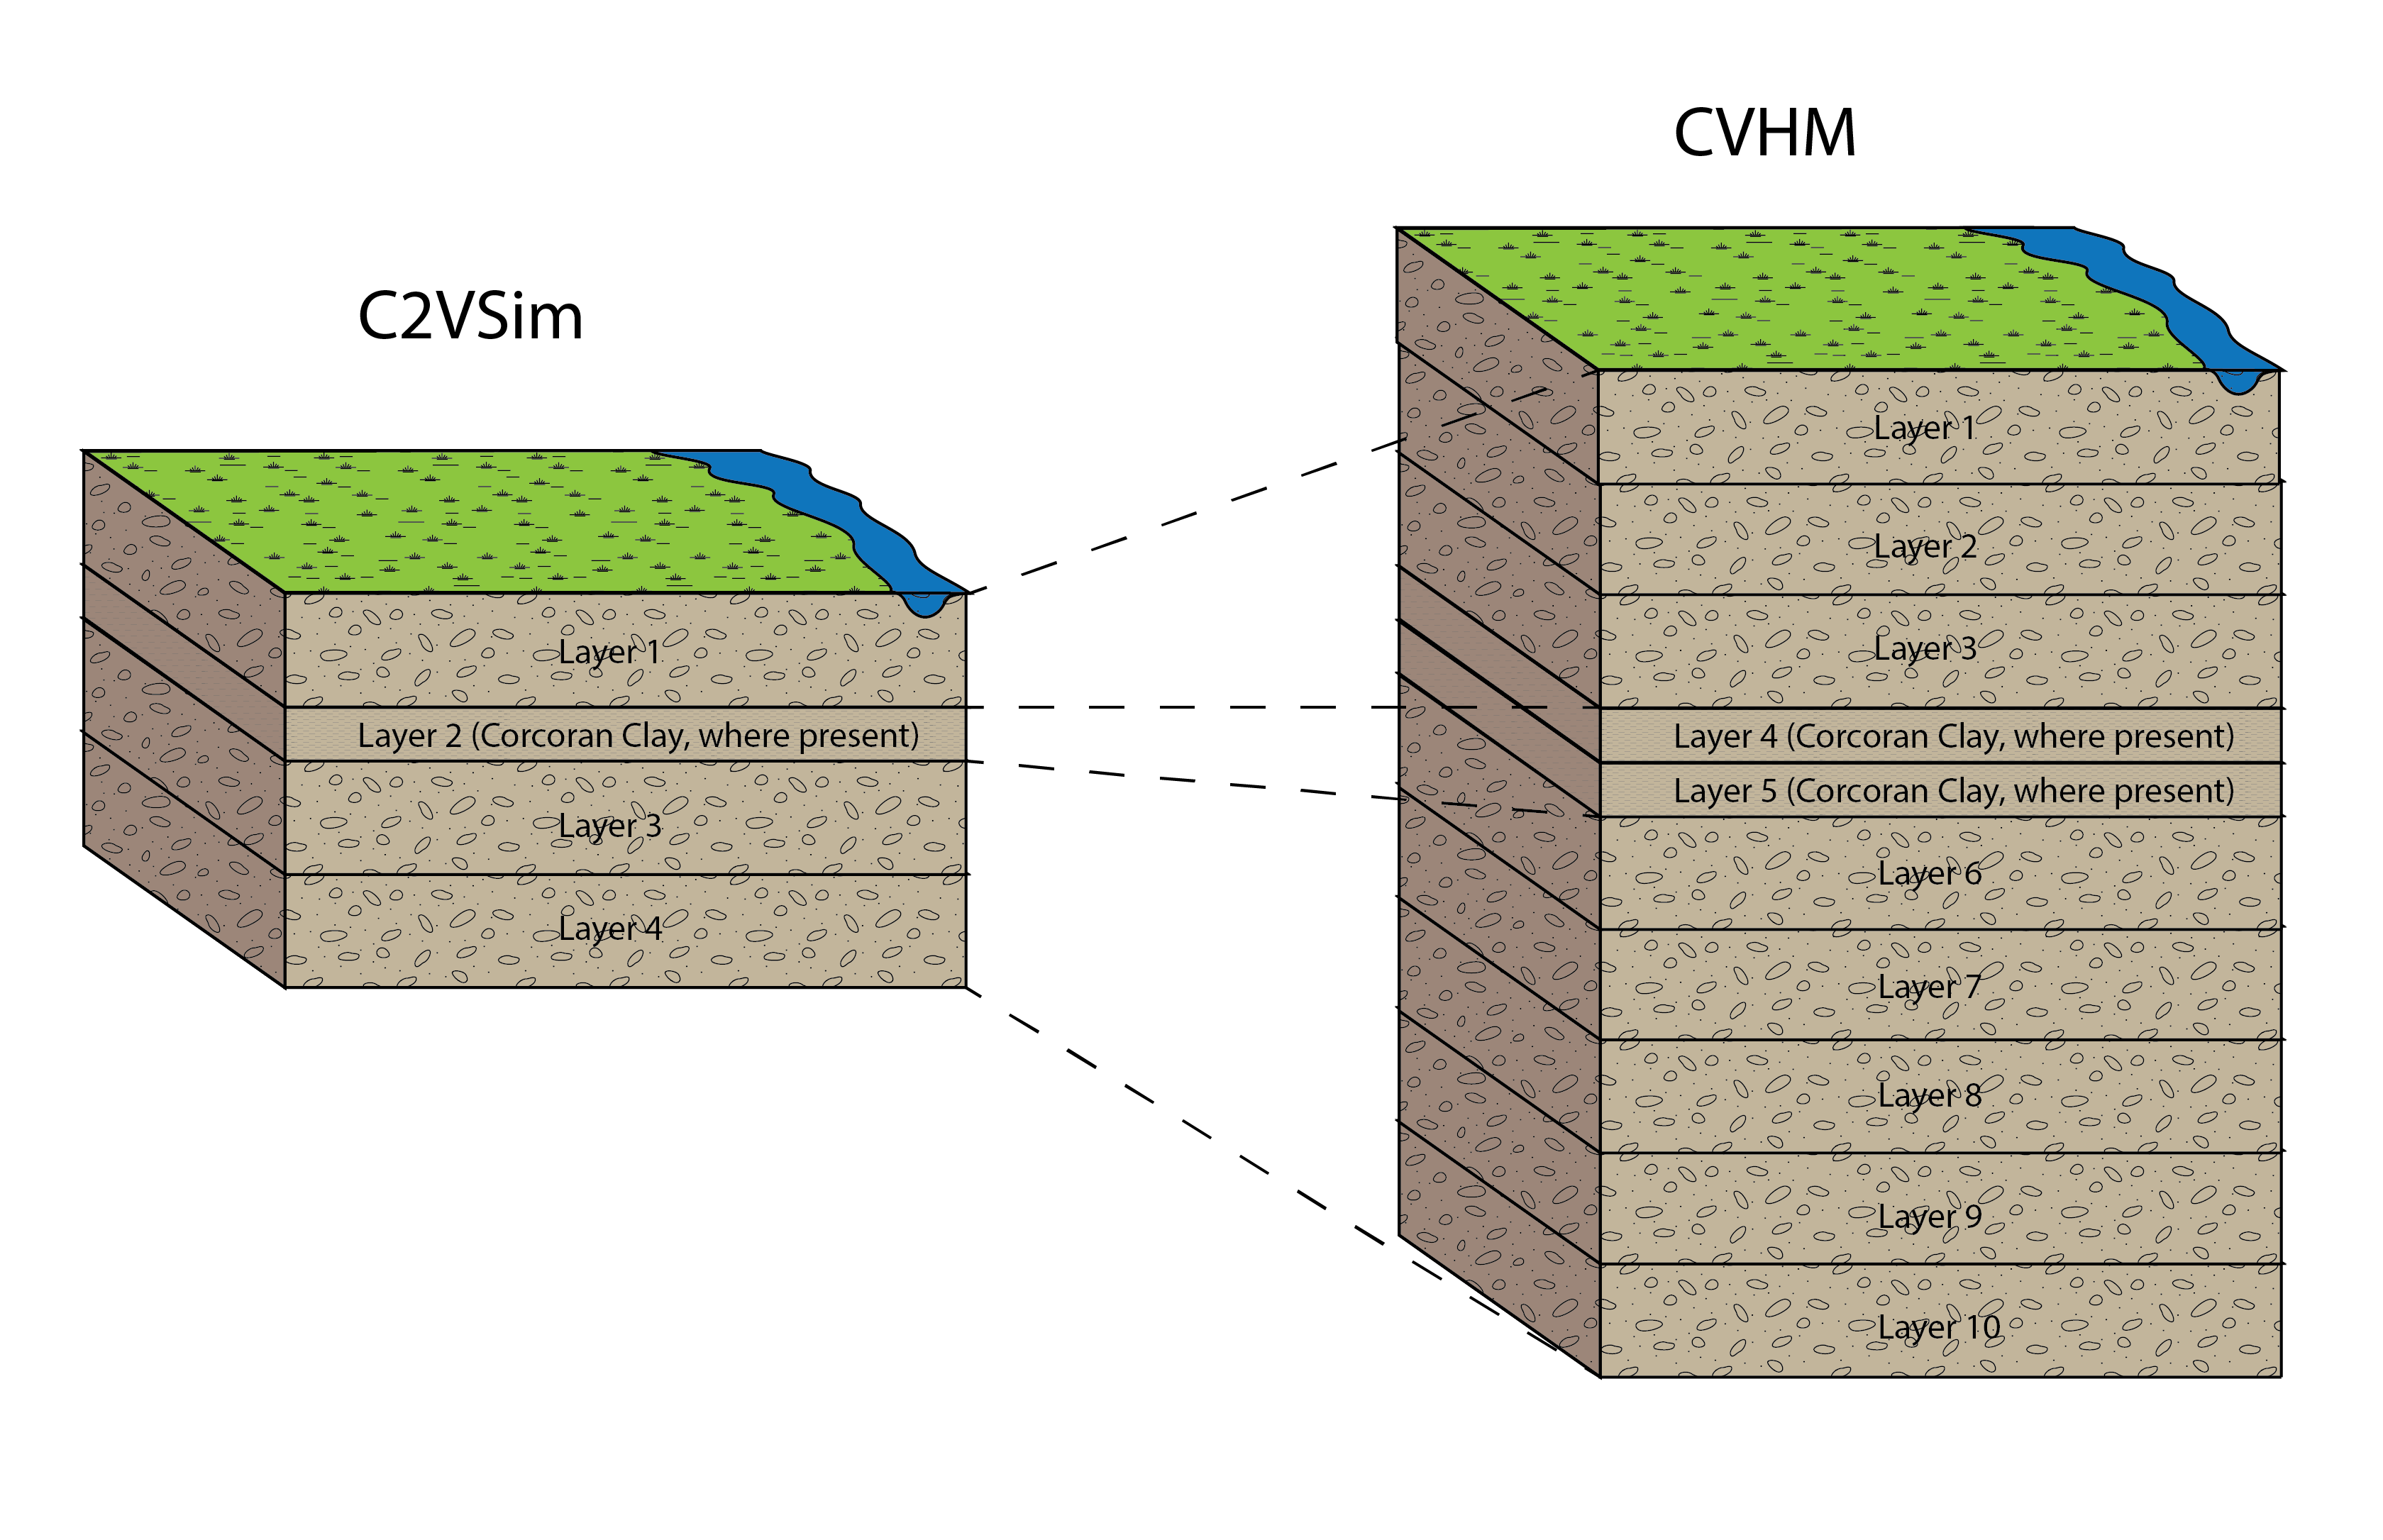
\includegraphics[width=140mm,keepaspectratio]{ch3_figs/GW_conceptualization.png}}
\caption{Groundwater model layers for CVHM and C2VSim. Coincident layers are indicated by dashed lines.}
\label{fig:ch3_model_layers}
\end{figure}

%%% RESULTS %%%
\section{Results}
\subsection{Major Landscape Water Budget Components}

Annual landscape water budget components were compared for CVHM and C2VSim at the supra-regional, regional, and sub-regional scales. Detailed comparisons of landscape water budget components for each of these regions are presented in Appendix \ref{app:compare_figs}. At the supra-regional scale (i.e., the entire Central Valley), the magnitudes of total fluxes into and out of the landscape were similar for each model (Fig. \ref{fig:LS_budget_SR26}). For both models, results show that the largest landscape water budget component into and out of the landscape were precipitation and ET, respectively, for the entire Central Valley. While the overall magnitudes of total fluxes out of the landscape were similar, results showed that C2VSim had a greater proportion of water leaving the landscape as runoff and return flows, while CVHM showed a greater proportion of deep percolation (Fig. \ref{fig:multi_LS_budget_SR26}c).

All statistical measures showed greater agreement for all landscape water budget components at the supra-regional and regional scales than for the subregional scales (Fig. \ref{fig:ch3_LS_components}). For example, average $RMSE$, $r$, and $|MBE|$ were 0.17, 0.83, and 0.15, respectively, for all water budget components at the supra-regional scale, 0.20, 0.73, and 0.17 at the regional scale, and 0.23, 0.67, and 0.19 at the subregional scale. Average $RMSE$ and $|MBE|$ were especially poor for water budget components in subregions 1--9 that comprise the Sacramento Valley and Delta and East Side Streams (i.e., $RMSE$ = 0.26 and $|MBE|$ = 0.23). For subregions comprising the San Joaquin and Tulare Lake regions in southern part of the Central Valley  (i.e., subregions 10--21) agreement was generally better (i.e., $RMSE$ = 0.19 and $|MBE|$ = 0.15). However, $r$ was greater for subregions 1--9 than for subregions 10--21 (i.e., $r$ = 0.71 and 0.56, respectively), which suggests that while the absolute agreement between water budgets in these subregions was general worse, the budget components typically showed similar interannual variations.

%% FIG LS components compare
\begin{figure}[ht!]
\centerline{\includegraphics[width=165mm,keepaspectratio]{ch3_figs/RMSE_r_bias_LS_082219.pdf}}
\caption{Statistical measures of correspondence, including normalized root mean square error (RMSE), pearsons $r$, and normalized mean bias for similar annual landscape water budget components for C2VSim and CVHM (1962-2003; horizontal axis) at the sub-regional, regional, and supra-regional scale (vertical axis). Landscape water budget components include precipitation in, surface water (SW) diversions in, and groundwater (GW) pumping in, runoff and return flows out, actual evapotranspiration ($ETa$) out, and deep percolation (i.e., recharge) out to the groundwater system.}
\label{fig:ch3_LS_components}
\end{figure}

Some individual water budget components showed particularly good agreement. Namely, precipitation had $RMSE$, $r$, and $|MBE|$ values of 0.03, 0.99, and 0.02, respectively. This is unsurprising given that precipitation is a model input rather than a simulated water budget component. Interestingly other model inputs like surface water diversions and evapotranspiration showed less agreement, despite that CVHM and C2VSim claim to use similar or identical datasets for land use and surface water inputs. Evapotranspiration showed good agreement for $RMSE$ and $|MBE|$ (0.15 and 0.11, respectively), but relatively poor correlation ($r$ = 0.43), suggesting that the overall magnitudes were similar, but the models showed less agreement for interannual and spatial variations. Surface water diversions, on the other hand, showed generally poor agreement for $RMSE$, $r$, and $|MBE|$ (0.30, 0.59, and 0.27, respectively), especially for subregions 1--9 in the northern Central Valley regions (0.38, 0.51, and 0.35, respectively).

Some systematic bias was shown for some water budget components, including runoff and return flow and deep percolation (Fig. \ref{fig:ch3_LS_components}). For all subregions, runoff and return flows were biased higher for C2VSim, while deep percolation was biased toward CVHM. These biases were especially pronounced for subregions 1--9 in the northern Central Valley regions.

In general, better agreement was observed for aggregated water budget components (i.e., Total in and Total out). These water budget components had  average $RMSE$, $r$, and $|MBE|$ of 0.13, 0.71, and 0.10, respectively, while those values for each of the water budget components that comprise the total fluxes averaged 0.26, 0.68, and 0.21 respectively. Finally, the statistical measures were generally consistent with each other, especially for $RMSE$ and $|MBE|$, so for example, if water budget comparison showed low $RMSE$, they typically also showed low $|MBE|$ and often high $r$ as well.

\subsection{Major Groundwater Budget Components}

Annual groundwater budget components were compared for CVHM and C2VSim at the supra-regional, regional, and sub-regional scales (Fig. \ref{fig:ch3_GW_components}). Detailed comparisons of groundwater budget components are presented in Appendix Section \ref{app:compare_figs}. Results show that the largest water budget components into and out of the groundwater system were landscape recharge and groundwater pumping, respectively (Fig. \ref{fig:GW_budget_SR26}) for the entire Central Valley. CVHM showed greater total flows into and out of the groundwater system as compared to C2VSim at the supra-regional scale (Fig. \ref{fig:multi_GW_budget_SR26}c), and regional scale for the Sacramento Valley (Fig. \ref{fig:multi_GW_budget_SR22}) and Delta and East Side Streams regions (Fig. \ref{fig:multi_GW_budget_SR23}), where flows into and out of the groundwater system were about 2$\times$ and 1.5$\times$ greater, respectively, for CVHM than for C2VSim.

Compared with landscape water budgets, groundwater budget components were generally more challenging to compare statistically because some water budget components contained insufficient measurements to calculate these statistics, especially for $r$ (Fig. \ref{fig:ch3_GW_components}b), which was not included in most subsequent analyses. In general, there was less agreement for groundwater water budgets than for landscape water budgets. Similar to the landscape water budgets, statistical measures showed slightly greater agreement for groundwater budget components at the regional scales than for the subregional scales. For example, average $RMSE$ and $|MBE|$ were 0.33 and 0.25, respectively, at the regional scale, and 0.35 and 0.27 at the subregional scale. However, agreement at the supra-regional scale was slightly worse than for the regional scale ($RMSE$ = 0.35 and $|MBE|$ = 0.30). Average $RMSE$ and $|MBE|$ were especially poor for water budget components in subregions 1--9 that comprise the Sacramento Valley and Delta and East Side Streams (i.e., $RMSE$ = 0.44 and $|MBE|$ = 0.37). For subregions comprising the San Joaquin and Tulare Lake regions in southern part of the Central Valley  (i.e., subregions 10--21) agreement was generally better (i.e., $RMSE$ = 0.28 and $|MBE|$ = 0.19). 

%% FIG GW components compare
\begin{figure}[ht!]
\centerline{\includegraphics[width=165mm,keepaspectratio]{ch3_figs/RMSE_r_bias_GW_082219.pdf}}
\caption{Statistical measures of correspondence, including normalized root mean square error (RMSE), pearsons $r$, and normalized mean bias for similar annual groundwater budget components for C2VSim and CVHM (1962--2003; horizontal axis) at the sub-regional, regional, and supra-wide scale (vertical axis). Groundwater budget components include gains from landscape recharge, gains from surface water leakage, gains from boundary flows in, losses from pumping, losses to groundwater discharge to surface water and the landscape, and losses from boundary flows out. Blank (white) boxes indicate instances where statistics could not be calculated due to insufficient data.}
\label{fig:ch3_GW_components}
\end{figure}

Some systematic bias was observed for some groundwater budget components (Fig. \ref{fig:ch3_GW_components}c). For example, total groundwater inflows and outflows were biased toward CVHM for most regions ($MSE$ = -0.17 and -0.18), indicating that there generally was more groundwater `throughput' in the CVHM groundwater system. Biases were especially large for subregions 1--9 in the northern Central Valley regions. For example, for model inflows, surface water gains and net boundary inflows had $MSE$ values of 0.27 and 0.23, showing bias toward C2VSim, but were offset by CVHM-biased landscape recharge ($MSE$ = -0.39). The strong CVHM bias in landscape recharge was similarly observed in the landscape budgets highlighted in the previous section. The compensatory effect of water budget components was apparent across scales for $RMSE$ and $MBE$. For example the average $RMSE$ and $|MBE|$ for \textit{Total in} and \textit{Total out} were 0.27, and 0.21, whereas the average $RMSE$ and $|MBE|$ for each of water budget components that comprise the total inflows and outflows were substantially greater (0.37 and 0.29, respectively).

Net boundary fluxes were calculated for all subregions to evaluate differences in groundwater flows and exchanges from model boundaries and adjacent subregions for each model. Surprisingly, 6 of 21 subregions showed opposite average net boundary groundwater fluxes during 1962--2003 (Fig. \ref{fig:ch3_GW_net_bound}). These discrepancies were especially pronounced in subregions 1--9 that comprise the northern Central Valley, where 5 of 9 subregions showed opposite signs, and the average discrepancies were 0.22 million acre-ft yr$^{-1}$ for these subregions. The magnitude of boundary flow discrepencies were somewhat less for subregions 10--21 that comprise the southern Central Valley (0.10 million acre-ft yr$^{-1}$, on average). 

%% FIG GW boundary flows
\begin{figure}[ht!]
\centerline{\includegraphics[width=85mm,keepaspectratio]{ch3_figs/net_bound_flows_no_reg.pdf}}
\caption{Annual average net boundary groundwater flux directions and magnitudes at the regional and subregional scales. CVHM and C2VSim fluxes are shown in orange and blue, respectively, in million acre-ft yr$^{-1}$ units.}
\label{fig:ch3_GW_net_bound}
\end{figure}

\subsection{Groundwater Storage Trends}

Average annual groundwater storage trends were calculated for each model at the supra-regional, regional, and sub-regional scales during 1962--2003 (Fig. \ref{fig:ch3_GW_delta_stor}a). To compare trends across spatial scales, annual volumetric change-in-storage trends were also converted to area-averaged values (Fig. \ref{fig:ch3_GW_delta_stor}b). For the area-averaged values, results show good agreement between models at the supra-regional scale, where differences in annual groundwater storage trends were $<$ 0.02 ft yr$^{-1}$. Average differences were progressively greater at the regional scale (0.08  ft yr$^{-1}$, on average) and subregional scale (0.13 ft yr$^{-1}$, on average). Interestingly, regional-scale change-in-storage discrepancies were smallest in the Sacramento Valley region (0.03 ft yr$^{-1}$), where other groundwater and landscape water budget components showed large discrepancies relative to other regions. Despite the small difference in the Sacramento Valley region groundwater storage trends, the directions of the trends for each model were opposite, i.e., CVHM showed a small overall increasing storage trend, while C2VSim showed groundwater losses. This type of behavior was also present in 6 of 21 subregions, namely those in the southern Sacramento and Delta and East Side Stream regions. The largest subregional trend discrepancies were for several subregions in the Tulare Lake region, where 3 subregions showed discrepancies $>$ 0.35 ft yr$^{-1}$. In general, we see a error compensation effect with scale for changes in groundwater storage, wherein larger local (i.e., sub-regional) discrepancies are partially mitigated as they are aggregated at larger spatial scales. When considering the volumetric change-in-storage trends for both models, it is notable that the average annual subregional change-in-storage magnitude for CVHM and C2VSim was 0.09 million acre-ft yr$^{-1}$ (Fig. \ref{fig:ch3_GW_delta_stor}a), which is less than the average annual subregional net boundary groundwater flow magnitude of 0.13 million acre-ft yr$^{-1}$ (Fig. \ref{fig:ch3_GW_net_bound}).

%% FIG GW delta stor
\begin{figure}[ht!]
\centerline{\includegraphics[width=160mm,keepaspectratio]{ch3_figs/delta_stor_discrepency_082619.pdf}}
\caption{(a) Total and (b) area-averaged groundwater change-in-storage trend (1962--2003) discrepancies for CVHM and C2VSim at the sub-regional, regional, and supra-regional (i.e., Central Valley-wide) scale.}
\label{fig:ch3_GW_delta_stor}
\end{figure}

\subsection{Groundwater Model Hydraulic Properties}

Hydraulic properties, including horizontal and vertical hydraulic conductivity ($K$) and storage properties were compared for coincident model layers at the supra-regional, regional, and sub-regional scales (Appendix \ref{app:compare_figs}). Results show substantial differences in hydraulic conductivity estimates between models (Fig. \ref{fig:ch3_hyd_prop_OOM}). The average order-of-magnitude difference in horizontal $K$ for the entire Central Valley was 0.73. Relatively good agreement was observed for horizontal $K$ in the uppermost model layers (order-of-magnitude difference $<$ 0.10), but differences were especially pronounced for horizontal $K$ in model layers underlying the Corcoran clay. Large discrepancies were observed for horizontal $K$ for the bottom-most coincident layers in each model (average order-of-magnitude difference = 1.57). The Central-Valley wide mean, median, and maximum horizontal $K$ were 446, 288, and 6636 ft d$^{-1}$, respectively, for CVHM layers 6--10 and were 43.1, 21.7, and 100 ft d$^{-1}$, respectively, for coincident layers 3--4 in C2VSim. Especially high horizontal $K$ values were specified for CVHM layers 6--10 in the Sacramento Valley region, where mean and median horizontal $K$ were 611 and 576 ft d$^{-1}$, respectively. Reported values of horizontal $K$ in layers 6--10 of CVHM are markedly outside the range of expected values for an alluvial aquifer system that is dominated by fine-texture facies \citep{anderson2015applied,botros2009spatial,fleckenstein2004managing,frei2009patterns,maserjian1993hydrogeologic,niswonger2008influence,sager2012effects}. Horizontal $K$ values were greater for all coincident layers in CVHM than for C2VSim in all but one subregion. 

Vertical $K$ agreement between models was generally better relative to the agreement for horizontal $K$. The average order-of-magnitude difference in vertical $K$ for the entire Central Valley was 0.45. For layers representing the Corcoran clay, which exert large control over vertical exchange between the shallow, semi-confined aquifer system and the deeper confined system in much of the southern Central Valley, CVHM and C2VSim median vertical $K$ values were similar (i.e., 1.5\times10$^{-4}$ and 7.1\times10$^{-4}$ ft d$^{-1}$, respectively).

%% FIG OOM difference in K
\begin{figure}[ht!]
\centerline{\includegraphics[width=75mm,keepaspectratio]{ch3_figs/hyd_prop_OOM_diff_082819.pdf}}
\caption{Order-of-magnitude differences in median horizontal and vertical hydraulic conductivity ($K$) for coincident layers and layer groups in C2VSim and CVHM. Blank (white) boxes indicate instances where a layer in either C2VSim or CVHM was not active.}
\label{fig:ch3_hyd_prop_OOM}
\end{figure}

\subsection{Unmeasured Agricultural Groundwater Pumping}

Average annual groundwater pumping discrepancies and percent differences in average annual groundwater pumping for CVHM and C2VSim are shown at the sub-regional, regional, and supra-regional scale (i.e., Central Valley-wide) during 1962–2003 (Fig. \ref{fig:ch3_GW_pumping}). Because specified urban groundwater pumping volumes are identical for each subregion in CVHM and C2VSim \citep{faunt2009groundwater}, any discrepancies in total groundwater pumping volumes are due to differences in estimated unmeasured agricultural groundwater pumping alone. Similar to other water budget components, substantial error compensation was observed as a function of spatial scale when comparing the percent differences in pumping volumes in each model (Fig. \ref{fig:ch3_GW_pumping}b). For example, the average groundwater pumping discrepancy between CVHM and C2VSim was 0.25 million acre-ft yr$^{-1}$ at the supra-regional scale (Fig. \ref{fig:ch3_GW_pumping}a), which amounts to only a 2\% difference between the total pumping volumes for the entire Central Valley (Fig. \ref{fig:ch3_GW_pumping}b). At the subregional scale, the average volumetric discrepancies were similar in magnitude to the Central Valley-wide discrepancies (i.e., 0.17 and 0.25, million acre-ft yr$^{-1}$, respectively) for subregions 1--9 and 10--21, which represent the northern and southern portions of the Central Valley. However, on average, these volumes represent a much larger fraction of the estimated pumping in each subregion (percent difference = 76\% and 54\%, respectively). The average subregional discrepancies were 0.22 million acre-ft yr$^{-1}$ (63\% average percent difference) for all subregions. From a volumetric standpoint, these differences are similar in magnitude to the volumetric discrepancies for net boundary groundwater flows at the subregional scale (0.18 million acre-ft yr$^{-1}$, on average).

%% FIG GW delta stor
\begin{figure}[ht!]
\centerline{\includegraphics[width=160mm,keepaspectratio]{ch3_figs/pumping_discrepency_082619.pdf}}
\caption{(a) Average annual groundwater pumping discrepancies and (b) percent differences in average annual groundwater pumping for CVHM and C2VSim at the sub-regional, regional, and supra-regional (i.e., Central Valley-wide) during 1962--2003.}
\label{fig:ch3_GW_pumping}
\end{figure}

%%% DISCUSSION %%%
\section{Discussion}

CVHM and C2VSim both estimate landscape and groundwater budgets in the Central Valley aquifer system during 1962--2003, using agricultural groundwater models that are conceptually different and fraught with uncertainties that have not been previously investigated. Results presented here review annual water budget components for each model for coincident regions in the Central Valley during 1962--2003 to help provide insight into two related questions. (1) To what extent can unmeasured water budget components (i.e., agricultural groundwater pumping) in agriculturally-dominated groundwater systems can be constrained with a combination of agricultural irrigation accounting methods and groundwater models? (2) Do methodological or conceptual differences between models contribute to differences in water budget estimates in CVHM and C2VSim? Absent measured data for important water budgets---specifically for agricultural groundwater pumping---both of these questions are challenging to answer with quantitative metrics alone, but some valuable insights are gained by considering several specific examples.

For example, results show that the discrepancies between annual estimated groundwater pumping are similar in magnitude to discrepancies for other groundwater and landscape water budget components. At the subregional scale, the average annual volumetric discrepancy between CVHM and C2VSim estimated groundwater pumping was 0.22 million acre-ft yr$^{-1}$. Compared with specified model inputs, which are derived from similar or identical observations, i.e., precipitation, surface water diversions, and ET, average annual volumetric discrepancies were 0.04, 0.26, and 0.21 million acre-ft yr$^{-1}$, respectively. This suggests that the propagation of error was not substantially amplified by the agricultural irrigation accounting methods in either CVHM and C2VSim. When comparing groundwater pumping discrepancies with discrepancies for other simulated model outputs, e.g., groundwater boundary flows and groundwater change-in-storage trends, average annual volumetric discrepancies for also similar in magnitude (0.18 and 0.13 million acre-ft yr$^{-1}$, respectively). Interestingly, average annual volumetric discrepancies were substantially greater for deep percolation estimates (i.e., 0.40 million acre-ft yr$^{-1}$), which is largely a function of irrigation efficiency, a seldom measured crop- and irrigation practice-dependent factor that that is represented with distinctly different approaches in CVHM and C2VSim. 

Results suggest that there is some systematic bias in how excess irrigation water is represented in CVHM and C2VSim. For example, in the landscape system, all subregions showed a greater proportion of excess irrigation as deep percolation in CVHM, while C2VSim showed a greater proportion of excess irrigation as runoff and return flow (Fig. \ref{fig:LS_budget_SR26}). This discrepancy is reflected in groundwater budgets as well, where C2VSim offsets the smaller proportion of deep percolation with greater recharge from surface water gains and boundary inflows (Fig. \ref{fig:GW_budget_SR26}). However, greater deep percolation CVHM is not completely offset by these flows in C2VSim. Instead, CVHM shows systematically greater inflows and outflows in the groundwater system as compared to C2VSim, especially for subregions 1--9 in the northern Central Valley (Fig. \ref{fig:GW_budget_SR22}, \ref{fig:GW_budget_SR22}). This behavior likely reflects the fact that vertical and (especially) horizontal $K$ are typically orders of magnitude greater in CVHM as compared to C2VSim, especially in the northern Central Valley, where horizontal $K$ values are outside the expected range of values for this type of system. This discrepancy in horizontal $K$ would benefit from additional scrutiny and calibration by the developers of CVHM. 

In general, greater differences were observed for landscape and groundwater budgets in the northern Central Valley. The author speculates that this behavior likely reflects the shallow water table depths in this region, which allow for more exchange between the groundwater and surface water systems. Results presented here suggest that areas with greater exchange of groundwater and surface water can amplify methodological differences and propagates errors and uncertainties. For example, Subregion 4, where the majority of crops are rice \citep{faunt2009groundwater} shows the greatest discrepancies for groundwater pumping (Fig. \ref{fig:ch3_GW_pumping}). In this subregion, C2VSim estimates that a substantial proportion of the landscape water budget is from groundwater pumping, while CVHM estimates effectively zero pumping \ref{fig:LS_budget_SR4} because most of the landscape water budget is satisfied from ET from groundwater. In areas with deeper groundwater levels, smaller differences in most water budget components likely reflect the fact that there are fewer feedbacks between the groundwater and landscape systems in those areas. These findings highlight the importance of gathering measurements of fluxes (e.g., ET and groundwater pumping), especially in areas with ample exchanges of water between the groundwater and landscape systems.

Results suggest that it may be possible to estimate groundwater pumping by agriculture with landscape water budget accounting methods alone in areas where there is little exchange of groundwater and surface water (i.e., in areas with deep groundwater tables). Similarly, changes in groundwater storage may be more readily estimated with uncoupled approaches in areas with deep groundwater tables for the same reasons. In areas with relatively shallow water table depths like subregions 1--9 in the northern Central Valley, coupled methods like CVHM and C2VSim likely have a greater potential for accurately predicting water budgets and accounting for groundwater/surface-water exchanges, but it remains to be seen whether CVHM or C2VSim methodologies are better suited absent more measurements of groundwater pumping. Other studies have shown the importance of groundwater table depth on feedbacks between groundwater and the landscape in agriculturally-dominated systems \citep{condon2014feedbacks, condon2014groundwater}. The author speculates that many of the large discrepancies in water budget components observed in this region reflect unrealistic conceptualization of the aquifer system in CVHM.

Results make clear that substantial error compensation occurs as a function of spatial scale when comparing these models. Discrepancies between water budgets are typically larger at the subregional scale that is important for water management. This is especially important in light of the 2014 passage of California’s Sustainable Groundwater Management Act (SGMA), which required the formation of local Groundwater Sustainability Agencies (GSAs), which oversee groundwater management in $>$ 40 distinct areas in the Central Valley alone. These GSAs are typically smaller than the 21 Central Valley subregions, and are typically delineated according to political, rather than hydrologic boundaries. There is substantial interest on the part of SGMA stakeholders to use water budget estimates from both CVHM and C2VSim, either directly or to provide boundary conditions or water budget data for a finer-resolution nested model to develop water budget estimates for GSAs. In the Central Valley, where there is substantial groundwater flow across GSA boundaries, these boundary flows into and out of GSA boundaries are an important consideration and a challenging water budget component to estimate. Results presented here show large discrepancies for boundary flows at the subregional scale, especially in the northern Central Valley, where 6 of 9 subregions showed average annual boundary flows with opposite signs. Results show that the average annual discrepancy for net boundary flows at the subregional scale is 0.18 million acre-ft yr$^{-1}$, which is similar in magnitude to discrepancies for one of the largest groundwater budget components---groundwater pumping---between models (0.22 million acre-ft yr$^{-1}$). It is likely that uncertain boundary flow estimates will be major points of contention between adjacent GSAs as the SGMA process moves forward, and results from this study suggest that CVHM and C2VSim alone may not be particularly helpful in constraining these estimates.

Interestingly, some differences were observed for input data that ostensibly are derived from similar or identical sources. While some model inputs, e.g., precipitation, showed small average annual discrepancies between models at the subregional scale (0.04 million acre-ft yr$^{-1}$), other inputs like surface water diversions, showed larger average annual discrepancies at this scale (0.26 million acre-ft yr$^{-1}$), especially in the northern Central Valley (0.35 million acre-ft yr$^{-1}$). ET, which is not necessarily a model input, but is informed by similar land use and climate data in each model, showed a similar magnitude of average annual discrepancies at the subregional scale (0.21 million acre-ft yr$^{-1}$) to discrepancies for surface water diversions.

Despite the limitations and uncertainties in water budget estimates from these models, coupled agricultural groundwater models will likely remain the predominant approach for constraining water budgets in agriculturally-dominated groundwater systems like the Central Valley. Recent work has highlighted the value of ex-situ satellite measurements of groundwater abstraction at the global scale. For example, the Gravity Recovery and Climate Experiment (GRACE) satellites have estimated dramatic groundwater depletion in the Central Valley \citep{famiglietti2011satellites} and elsewhere \citep[e.g.,][]{rodell2009satellite,scanlon2012groundwater,scanlon2015hydrologic} during recent decades using remotely-sensed gravity measurements coupled with models; however, these ex-situ gravity measurements lack spatial and temporal resolution to adequately estimate groundwater storage changes on the monthly time scales that are important for water management \citep{alley2015bringing}. Indeed, a single GRACE pixel (about 77,000 sq. miles) \citep{famiglietti2011satellites} exceeds the total area of the Central Valley several times over, complicating attempts to isolate storage changes there. Given these limitations, coupled groundwater and agricultural surface-water models will likely continue to see widespread use for simulating groundwater response to irrigation demand and for estimating regional and sub-regional water budgets. 

%%% FUTURE WORK %%%
\section{Future Work}

Methodological differences between MF-MFP2 and IWFM and conceptual and parameterization differences in CVHM and C2VSim cannot be entirely separated with the comparisons presented here. In order to fully understand the degree to which differences in water budget estimates reflect propagation of the inherent parametric uncertainty of input data (i.e., data on crops, weather and climate, and surface water deliveries) or structural uncertainty of the methods, a more targeted approach in which MF-FMP2 and IWFM methods are separately applied to a groundwater basin in which the major water budgets are well known. For example, the Pajaro groundwater basin along the California coast has, for decades, collected comprehensive groundwater pumping data and detailed groundwater head data. A model using an the MF-FMP2 approach has already been developed for the region \citep{hanson2012method}. Future research could, in theory, develop a companion model using the same land use, geology, and water budget input data with the IWFM approach to help tease out whether methodological differences between approaches contribute to differences in estimated water budgets for this system.

%%% CONCLUSIONS %%%
\section{Conclusions}

Accurate estimation of groundwater budgets and effective management of agricultural groundwater pumping in California’s Central Valley is a priority for achieving new, legally-mandated groundwater management goals. Comprehensive measurements of agricultural groundwater pumpage in the Central Valley are uncommon, despite that this is typically one of the largest components of the groundwater budget. Without these measurements, accurate estimation of groundwater budgets remains a challenge in much of the Central Valley. CVHM and C2VSim are two regional-scale hydrologic models that couple groundwater and agricultural water budget models to provide historical and current estimates of groundwater and landscape water budgets in the Central Valley. However, both models estimate these water budget components using conceptually different representations of the agricultural landscape system. This work reviews groundwater and landscape water budgets for coincident areas in the Central Valley at the supra-regional, regional, and sub-regional scale during a concurrent 42-year simulation period from 1962--2003. 

Results showed wide-ranging, and sometimes large differences in the magnitude of simulated water budget components between models, with generally better agreement at larger spatial scales and for aggregated water budget components. Agreement of water budget components was relatively poor at sub-regional scales that are important for water management, especially in the northern Central Valley region, where major aquifer-conceptualization discrepancies are observed. Improved agreement observed at larger spatial scales reflects an error compensation effect. Systematic biases reflecting the partitioning of outflows from the landscape systems were observed between models, likely reflecting conceptual differences in the process representation of the soil zone system. Some differences were also observed for input data that ostensibly are derived from similar or identical sources and likely contribute to differences in simulated output discrepancies. These findings have important implications for the utility of these models for estimating water budgets for recently-passed groundwater legislation in California.

\section{Acknowledgements}
We gratefully thank Alvar Escriva-Bou, Emin Dogrul, Claudia Faunt, Charlie Brush, Jonathan Traum, Rich Niswonger, and Gus Tolley for their assistance. Support for this research was provided by the National Science Foundation (NSF) Climate Change, Water, and Society (CCWAS) Integrated Graduate Education and Research Traineeship (IGERT) program at the University of California, Davis and Colorado School of Mines (http://ccwas.ucdavis.edu, DGE-10693333) (SM, GF, RM), the NSF Graduate Research Fellowship (SM), the University of California Water (UC Water) Security and Sustainability Research Initiative (SM, GF, LF). All data used in the analysis can be made available by SM (srmap@ucdavis.edu).